\documentclass{article}
\usepackage{graphicx} % Required for inserting images

\title{Problem Set 6}
\author{Murphy Chesley}
\date{March 2026}

\begin{document}

\maketitle

\section{Data Explanation and Cleaning}

For this problem set, I decided to pull information from the Environmental Protection Agency's 2023 data summary spreadsheets. These spreadsheet provide data over facilities in the Greenhouse Gas Reporting system. Total emissions, industry type, location, and type of emitter are recorded each year beginning in 2010. 

I want to look and see if there had been any changes in GHG emissions stemming from the Obama Administration's 2015 Clean Power Plan. To do this, I first read the file in and cleaned the column names as the original column names had uppercase letters and spaces. I used the clean\_names() function to do this. I then wanted to get aggregate data for each of the states, so I separated the data by states and totaled their facilities' combined emissions. I wanted to put the total into a clean table, so I combined the data frames using the bind\_rows() function and made them wide format using pivot\_wide(). 

For the graphing portion, I first needed to partition the data by region instead of states as a graph with each state would be difficult to read and have far too much going on. In addition, there are also some wide gaps between high emitting states, such as Texas, and low emitting states, such as Vermont. The scale would be difficult to understand and needed to be grouped for clarity.


\section{Northeast Region}
\begin{figure}[h]
    \centering
    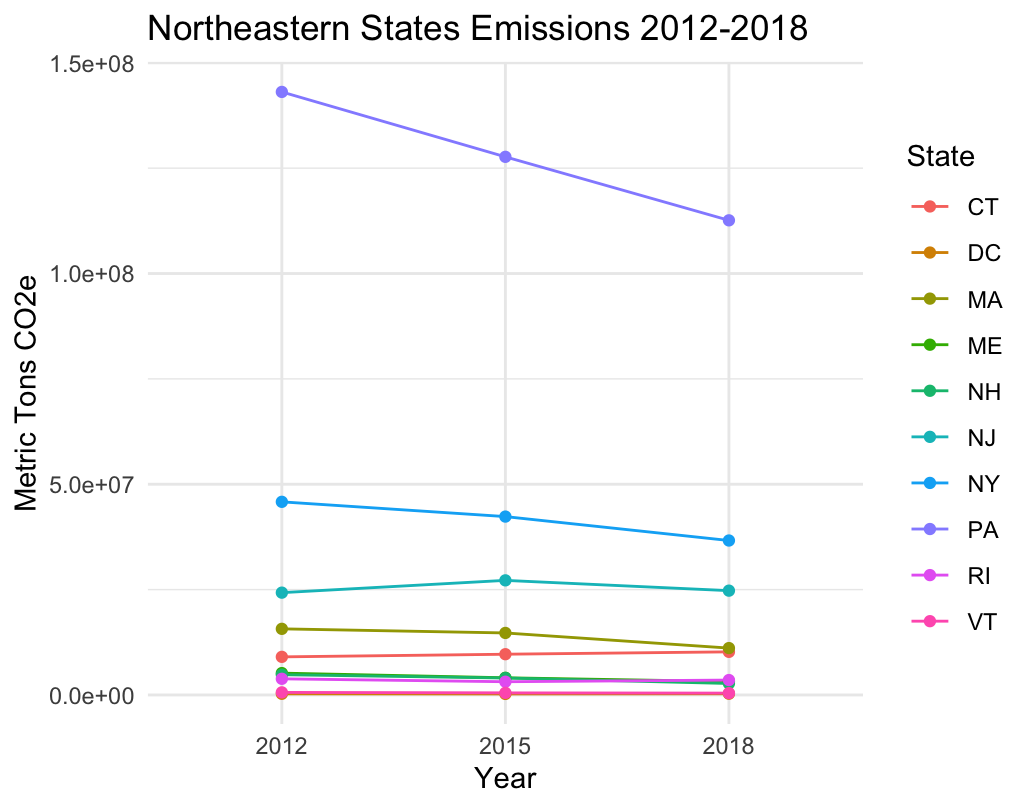
\includegraphics[width=0.8\textwidth]{PS6a_Chesley.png}
\end{figure}

The above graph shows the total emissions from facilities in states in the Northeastern region of the US for 2012, 2015, and 2018. This graph is measured in metric tons and uses scientific notation to show the scale of emissions. In this graph, we can see that Pennsylvania emits 150 million metric tons of GHG each year. This will be useful as it shows how states in the northeast region possibly responded to the Clean Power Plan. 

\section{South Region}
\begin{figure}[h]
    \centering
    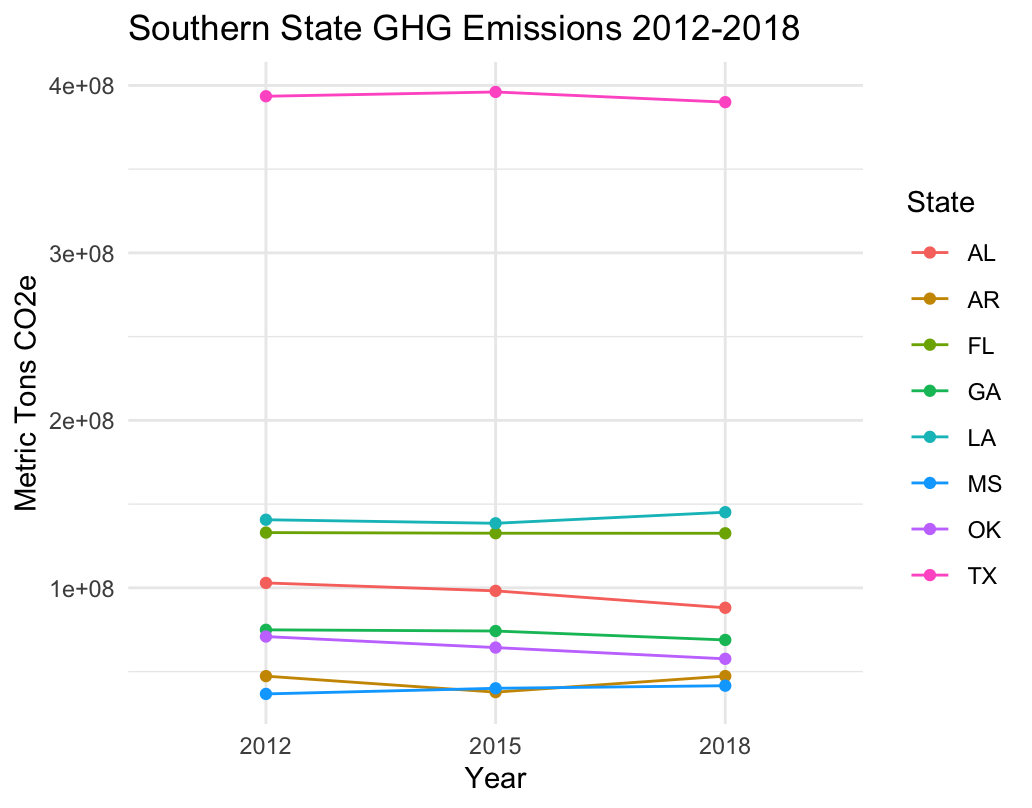
\includegraphics[width=0.8\textwidth]{PS6b_Chesley.png}
\end{figure}

The above graph shows the total emissions from facilities in the southern states. This is one of the larger regions, so emissions tend to be higher than the other regions in general. We see that there are not a lot of changes in this region and for some states, their emissions rose after 2015. This has many explanations, but further research will be needed to understand that better. This graph will help to understand possible regional differences in the data set, particularly with how GHG emissions are connected to industry.

\section{Midwest Region}
\begin{figure}[h]
    \centering
    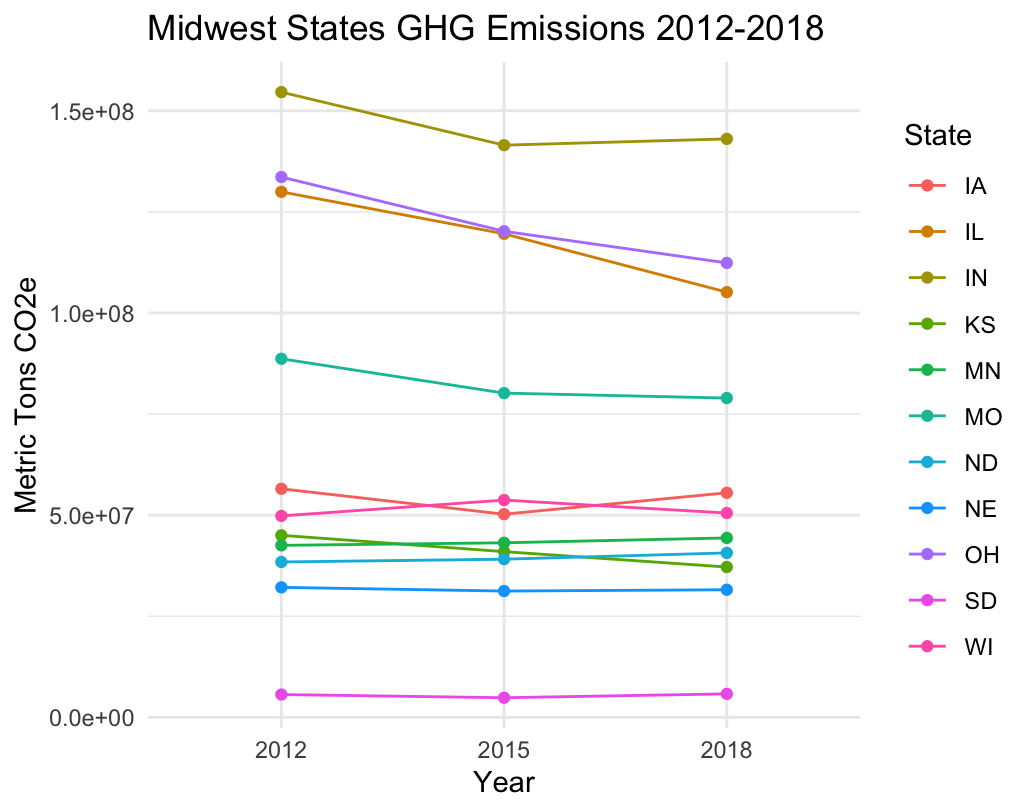
\includegraphics[width=0.8\textwidth]{PS6c_Chesley.png}
\end{figure}

The last graph here shows the total emissions from facilities in the midwestern states. These states are highly industrialized states which have varying degrees of GHG emissions. Some of the states, particularly Ohio and Illinois seemed to respond well after 2015, but further research will need to be done to see if this is related to the Clean Power Plan. 

\end{document}
